% FONTE TEMA https://github.com/matze/mtheme
\documentclass[aspectratio=1610]{beamer}
%\documentclass[aspectratio=1610, handout]{beamer}
\usepackage[utf8]{inputenc}
\usepackage{ragged2e}
\usepackage{xcolor}
\usepackage[italian]{babel}
\usepackage{multirow}
\usepackage{silence}
\WarningFilter{beamer}{}
\WarningFilter{metropolis}{}
\usetheme[progressbar=frametitle,titleformat=smallcaps]{metropolis}
\setbeamertemplate{frame numbering}[fraction]
\setbeamercovered{dynamic}
\definecolor{rosso}{RGB}{255, 0, 0}
\definecolor{giallo}{RGB}{254,212,23}
\hypersetup{colorlinks=true,linkcolor=black,urlcolor=rosso}
\setbeamercolor{palette primary}{fg=black, bg=giallo}
\setbeamercolor{background canvas}{bg=white}
\setbeamercolor{normal text}{fg=black}
\setbeamercolor{progress bar}{fg=rosso}
\setbeamercolor{framesubtitle}{fg=rosso}
\setbeamercolor{normal text .dimmed}{fg=giallo}
\setbeamercolor{block title alerted}{fg=rosso, bg=giallo}
\setbeamerfont{caption}{size=\tiny}
\setbeamerfont{caption name}{size=\tiny}
\setlength{\abovecaptionskip}{0pt}
\makeatletter
\metroset{block=fill}
\setlength{\metropolis@progressinheadfoot@linewidth}{1pt} 
\setlength{\metropolis@progressonsectionpage@linewidth}{1pt}
\setlength{\metropolis@titleseparator@linewidth}{1pt}
\makeatother

\title{TRADUZIONE MODELLO ER}
\subtitle{Regole di conversione}
\date{}
\institute{\textit{
        Fonti:
        \begin{itemize}
            \item[-] \href{https://it.wikipedia.org/wiki/Modello_E-R}{Wikipedia}
        \end{itemize}
    }
}

\begin{document}

\begin{frame}[plain, noframenumbering]
    \titlepage
\end{frame}

\begin{frame}{REGOLE DI CONVERSIONE}
    \begin{figure}
        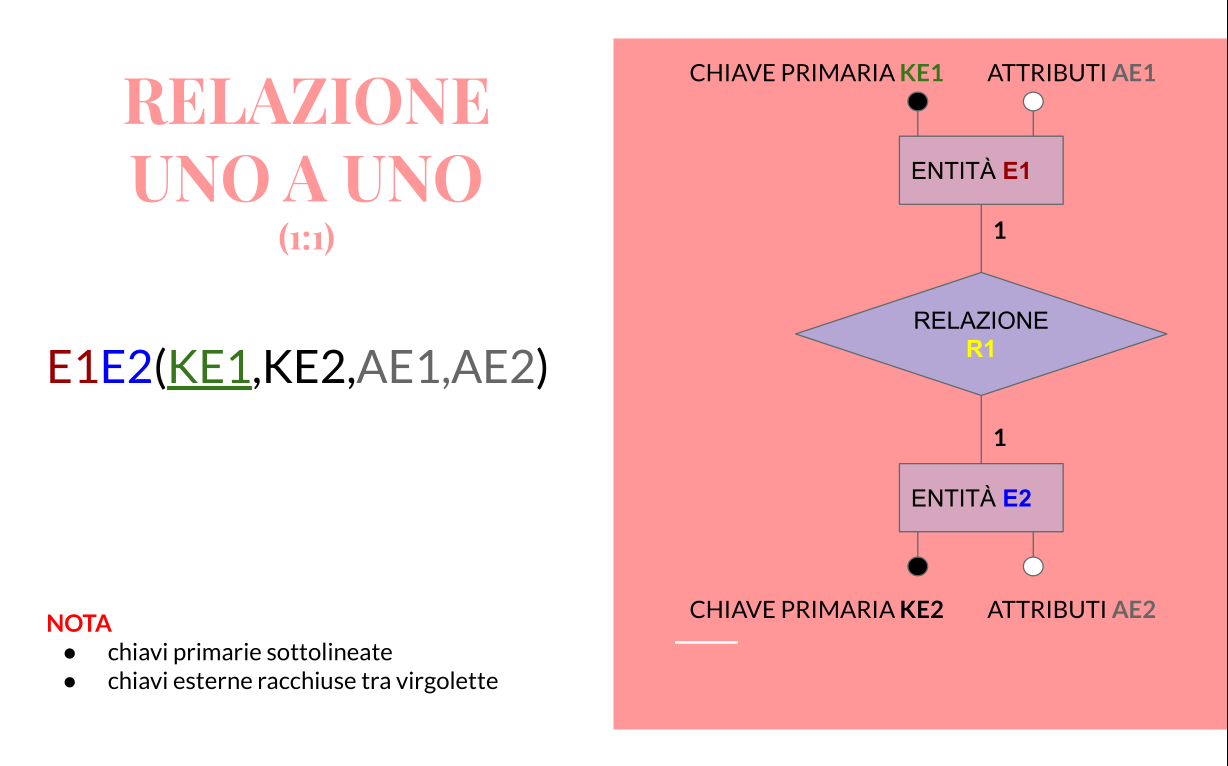
\includegraphics[width=.9\linewidth]{img/unoAuno.png}
        \caption{{creata con \href{https://docs.google.com/presentation/}{Google Slides}}}
    \end{figure}
\end{frame}

\begin{frame}{REGOLE DI CONVERSIONE}
    \begin{figure}
        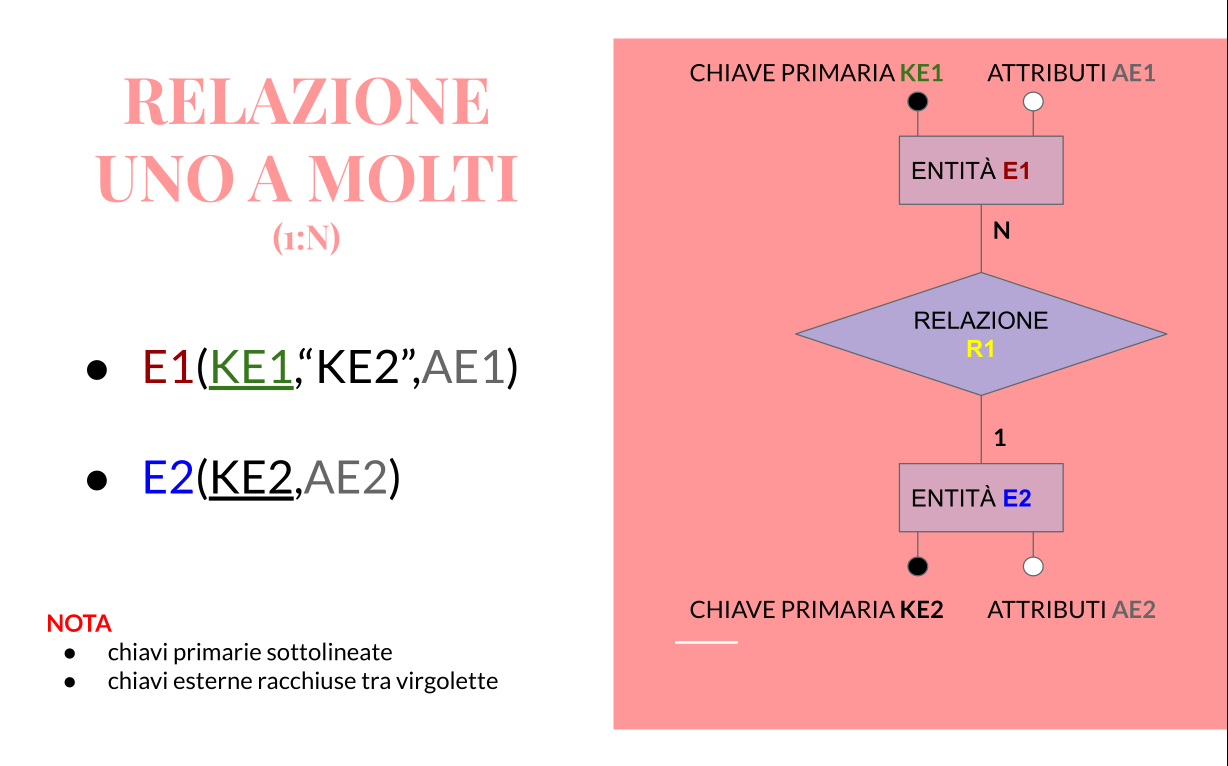
\includegraphics[width=.9\linewidth]{img/unoAmolti.png}
        \caption{{creata con \href{https://docs.google.com/presentation/}{Google Slides}}}
    \end{figure}
\end{frame}

\begin{frame}{REGOLE DI CONVERSIONE}
    \begin{figure}
        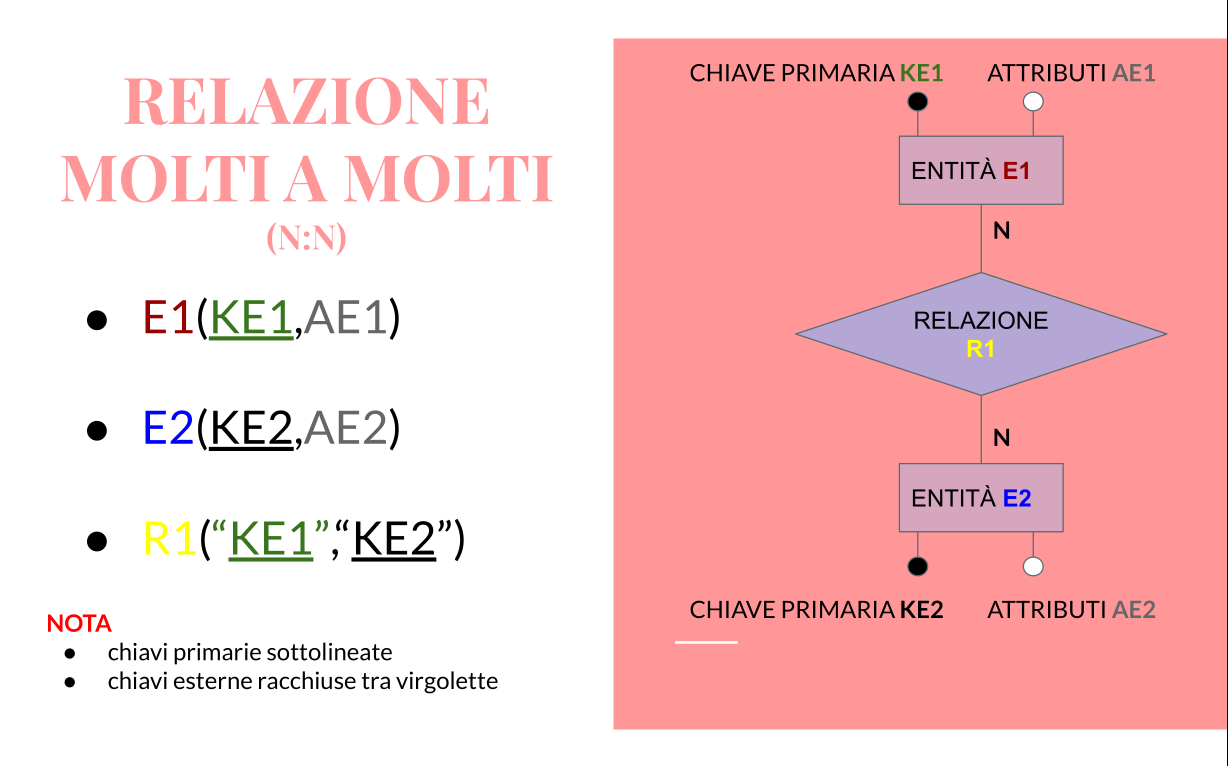
\includegraphics[width=.9\linewidth]{img/moltiAmolti.png}
        \caption{{creata con \href{https://docs.google.com/presentation/}{Google Slides}}}
    \end{figure}
\end{frame}

\end{document}